%!TEX TS-program = xelatex
%!TEX encoding = UTF-8 Unicode
\documentclass[11.5pt]{beamer}
%\usepackage{pgfpages}
%\pgfpagesuselayout{4 on 1}[a4paper,border shrink=5mm]

\usepackage[english]{babel}
%\usepackage[utf8x]{inputenc}

% mathmatical fonts and formulations
\usepackage{amsfonts}
\usepackage{amsmath}
\usepackage{amsthm}
\usepackage{amssymb}
% float control
\usepackage{placeins}
% graphic control
\usepackage{pgf}
\usepackage{tikz}
\usepackage{xcolor}
% Algorithm support
%\usepackage{algorithmic}
\usepackage{algorithm2e}
%color of the word
\usepackage{color}
% change the counter of enumerate
\usepackage{enumerate}
\usepackage{fix-cm}

\usepackage{mathspec}


%\usepackage{fontspec,xltxtra,xunicode}
\defaultfontfeatures{Mapping=tex-text}
%\setsansfont[Scale=MatchLowercase,Mapping=tex-text]{Comic Sans MS}

%\setmathsfont(Digits,Latin,Greek)[Numbers={Lining,Proportional}]{Comic Sans MS}

\mode<presentation>
{
  \usetheme{default}      % or try Darmstadt, Madrid, Warsaw, ...
  \usecolortheme{default} % or try albatross, beaver, crane, ...
  \usefonttheme{default}  % or try serif, structurebold, ...
  \setbeamertemplate{navigation symbols}{}
  \setbeamertemplate{caption}[numbered]
  \setbeamertemplate{footline}[frame number]
} 
\setbeamertemplate{frametitle}{
	\vspace{1em}
	\begin{center}{
	\Huge{\insertframetitle}
	}
	\end{center}
}



\title{COMP3721 Tutorial 8}
\author{}
\institute{CSE, HKUST}
\date{\today}

\begin{document}

\begin{frame}
  \titlepage
\end{frame}

\begin{frame}[t]
\frametitle{Problem 1}
\begin{enumerate}[(1)]
\item Knowing that $M = (K,\Sigma, \delta, s, H)$, give the mathematical definition of the following Turing machine.
\begin{center}
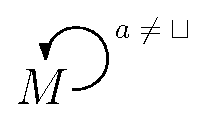
\includegraphics[scale = 0.6]{q1.eps}
\end{center}

\vspace{2em}
\uncover<2>{
Solution:

$M' = (K', \Sigma, \delta', s, \{h'\})$ where
\begin{itemize}
\item $K' = K\cup\{h'\}$
\item $\delta' = \delta\cup\{\text{$(h,a,s,a)$ : $h\in H$, $a\neq \sqcup$}\}\cup\{\text{$(h,\sqcup, h',\sqcup)$}\}$
\end{itemize}
}
\end{enumerate}
\end{frame}


\begin{frame}[t]
\frametitle{Problem 2}
\begin{enumerate}[(2)]
\item Explain what this machine does on the input $\triangleright\underline{\sqcup} w$.
\begin{center}
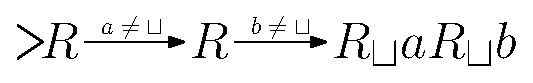
\includegraphics[scale = 0.6]{q2.eps}
\end{center} 

\vspace{2em}
\uncover<2>{
Solution:

If $|w|\geq 2$, then this machine copies the first two symbols of $w$, and paste them to the end of $w$.
}
\end{enumerate}
\end{frame}

\begin{frame}[t]
\frametitle{Problem 3}
\begin{enumerate}[(3)]
\item Trace the operation of the following Turing machine when started on $\triangleright{\sqcup} aabb\underline{\sqcup}$.
\begin{center}
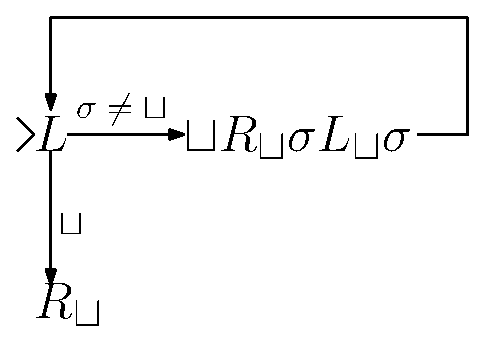
\includegraphics[scale = 0.6]{q3.eps}
\end{center}

\vspace{2em}
\uncover<2>{
The output is $\triangleright{\sqcup} aabbbbaa\underline{\sqcup}$
}
\end{enumerate}
\end{frame}
\end{document}
